\documentclass{extbook}
\usepackage[papersize={8.5in,11in},top=1in,bottom=1in]{geometry}
\RequirePackage{fix-cm}
\usepackage[T1]{fontenc}
\usepackage{lmodern}
\usepackage{fullpage}
\usepackage{titlesec}
\usepackage{parskip}
\usepackage{float}
\usepackage{url}
\usepackage{hyperref}
\usepackage{graphicx}
\usepackage{listings}
\usepackage{tcolorbox}
\usepackage{tabularx}
\usepackage{xcolor}
\usepackage{titlesec}
\usepackage{amsmath}
\usepackage{pdfpages}
\usepackage[utf8]{inputenc}
\usepackage{animate}
\usepackage{xmpmulti}
\usepackage{movie15}
%\usepackage{fancyhdr}

%renombro de ingles a español
\renewcommand{\contentsname}{Contenido}
\renewcommand{\figurename}{Figura}
\renewcommand{\listfigurename}{Lista de figuras}
\renewcommand{\bibname}{Bibliografía}
\renewcommand{\tablename}{Tabla}
\renewcommand{\listtablename}{Lista de tablas}


\usepackage[fontsize=13.5pt]{fontsize}
\setlength{\parindent}{0pt}

\titleformat{\chapter}[display]
  {\bfseries\huge} % Estilo del título
  {\hfill\Large} % Alineación a la derecha
  {3ex} % Espaciado entre el número del capítulo y el título
  {\vspace{-5cm}\titlerule\vspace{1.5ex}\hfill} % Regla arriba y alineación del título a la derecha
  [\vspace{1ex}\titlerule] % Regla debajo del título


  \makeatletter
  \patchcmd{\chapter}
    {\if@openright\cleardoublepage\else\clearpage\fi}
    {\clearpage}
    {}{}
  \makeatother


\begin{document}
\thispagestyle{empty}
\begin{minipage}{.15\textwidth}
  \flushleft
  \center{
\includegraphics[scale=0.035]{Imagenes/utp.png}}

  \vspace{20pt}

  \center{
    \rule{.5pt}{.6\textheight}
    \hspace{7pt}
    \rule{2pt}{.6\textheight}
    \hspace{7pt}
    \rule{.5pt}{.6\textheight}
  } \\

  \center{
\includegraphics[scale=0.28]{Imagenes/fisc.png}}
\end{minipage}
\begin{minipage}{.7\textwidth}
\flushright

\center{
  \center{
    \LARGE{U}\large{NIVERSIDAD} 
    \LARGE{T}\large{ECNOLÓGICA} \\[10pt]
    \large{DE} 
    \LARGE{P}\large{ANAMÁ} 
  } \\
  \rule{\textwidth}{2pt}
  \\
  \hrulefill\\[.5cm]
  
  \center{
    \LARGE{F}\large{ACULTAD DE } \LARGE{I}\large{NGENIERÍA} \LARGE{D}\large{E}\\[0.35cm]
    \LARGE{S}\large{ISTEMAS} \LARGE{C}\large{OMPUTACIONALES}\\[1cm]

    \LARGE{C}\large{ENTRO} \LARGE{R}\large{EGIONAL} \LARGE{D}\large{E} \LARGE{V}\large{ERAGUAS}\\[1cm]

  }


  \rule{\linewidth}{0.75mm}\\
  {\Large \textsc{Parcial N° 3: Simuladores de Robótica}}\\[0cm]

  \rule{\linewidth}{0.75mm}\smallskip

  \large{PRESENTA:}\\[0.3cm]

  \large{ \textbf{
  PUGA, ELBIN\\
  ORTEGA, PRISCILA\\
  BARRERA, ARLAND}
   }\\[0.5cm]

  \large{
TUTOR  }\\[0.35cm]

  \large{
\textbf{DR. CRISTIAN PINZÓN TREJOS}}
}\\[1cm]

  \large{
2024
}
\end{minipage}
\tableofcontents
\listoffigures
\listoftables
\chapter{Introducción}
\input{introducción.tex}
\chapter{ZMROBO}
\begin{figure}[H]
    \centering
    
\includegraphics[scale = 0.50]{Imagenes/zmobot_logo.png}
    \caption{Logo de ZMROBOT}{Fuente: Adaptado de ~\cite{zmrobo}}
\end{figure}

Fundada en 2002, ZMROBO tiene la misión de "crear una era inteligente con los estudiantes". Es una subsidiaria de Sheng Tong Shares. La empresa ofrece una amplia gama de productos educativos para estudiantes de todas las edades, incluidos hardware y software de robótica, planes de estudio, soluciones educativas K12 y servicios de personalización profesional.
ZMROBO permite a los usuarios construir fácilmente sus robots únicos con bloques y experimentar la diversión de crear con IA. ZMROBO tiene como objetivo despertar el interés de los jóvenes en la robótica a través de nuestros esfuerzos continuos, y los alentamos a participar en eventos creativos para mejorar su alfabetización y mentalidad y explorar el mundo del futuro ~\cite{zmrobo}.

\chapter{ROBOSIM}
\begin{figure}[H]
    \centering
    
\includegraphics[scale = 0.50]{Imagenes/robosimlogo.png}
    \caption{Logo de Robosim}{Fuente: Adaptado de ~\cite{robosim}}
\end{figure}

RoboSim es un software de aprendizaje de robótica virtual desarrollado por ZMROBO que combina conocimientos multidisciplinarios de inteligencia artificial, física, simulación 3D y computación, para que los estudiantes puedan realizar la educación y creación de robots en un entorno virtual de computadora, participar en varias competiciones en línea y otras actividades, completar diferentes niveles de aprendizaje, capacitación y competencia en inteligencia artificial y educación en programación, a fin de mejorar su capacidad en STEAM y aspectos integrales.

Para ampliar las capacidades de los robots, RoboSim fue desarrollado para proporcionar a los estudiantes robots virtuales cuando los robots físicos no están disponibles. El esquema de control para los robots virtuales es idéntico al físico. La GUI se utiliza para posicionar robots y obstáculos dentro de la simulación para que el estudiante pueda tener una referencia visual de la configuración ~\cite{gucwa2}.

\subsection{Características}
\input{características.tex}

\subsection{Instalación de la plataforma}
\input{instalación_de_la_plataforma.tex}

\subsection{Interfaz de Usuario}
La interfaz principal de RoboSim se ve de esta manera: 

\begin{figure}[H]
    \centering
    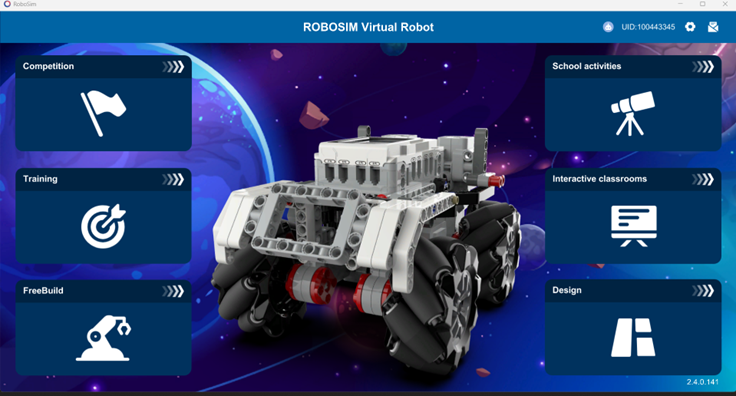
\includegraphics[scale = 0.70]{Imagenes/interfaz1.png}
    \caption{Interfaz principal del software}{Fuente: Propia}
\end{figure}

En donde podemos apreciar las diferentes opciones que nos ofrece este software de simulación

\textbf{Competencia en línea:} Muestra las competencias disponibles. Al hacer clic en una competencia específica, podrás ver el registro y acceder al lugar del evento.

\textbf{Entrenamiento temático:} Ofrece espacios de práctica basados en distintos temas de competencia.

\textbf{Construcción libre:} Permite construir el robot sin restricciones y guardar los archivos de construcción en tu computadora.

\textbf{Recursos del curso:} Diseñados para adaptarse a los materiales utilizados en RoboSim.

\textbf{Diseño de lugares:} Crea y edita espacios de entrenamiento de manera independiente.


\newpage

\subsection{Opciones disponibles}
Construcción Tridimensional

\begin{figure}[H]
    \centering
    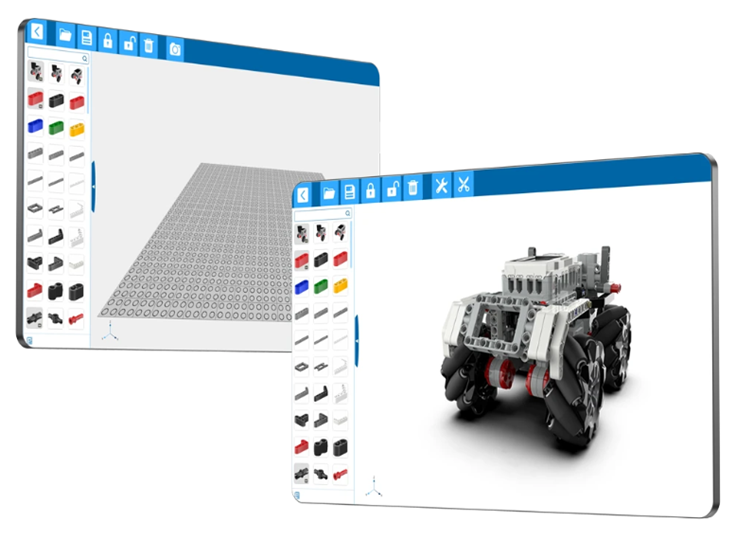
\includegraphics[scale = 0.50]{Imagenes/trid.png}
    \caption{Construcción en 3 dimensiones}{Fuente: Propia}
\end{figure}

\textbf{Columna de bloques de construcción:} Se utiliza para seleccionar los bloques de construcción necesarios. Hay 10 categorías que incluyen robots, vigas, pasadores, ejes, engranajes, componentes electrónicos, piezas decorativas, casquillos, ruedas y otros.

\textbf{Barra de búsqueda:} Puede buscar los bloques de construcción correspondientes ingresando sus nombres.

\textbf{Abrir archivo:} Abra el archivo del modelo de robot en la computadora. El formato de archivo que se puede abrir es rsr.

\textbf{Guardar archivo:} Guarde el modelo del robot en la computadora, el formato de archivo es rsr.

\textbf{Congelar bloques de construcción:} Congele los bloques de construcción seleccionados para que no participen en la coincidencia de adsorción.

Para este modo de construcción libre el software nos da una serie de herramientas como pueden ser: llantas, robots, pin, ejes, engranaje y manguito del eje ~\cite{chino}.

\begin{figure}[H]
    \centering
    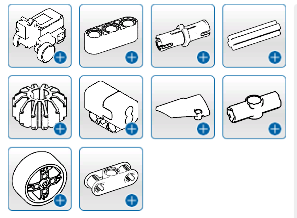
\includegraphics[scale = 0.95]{Imagenes/herramientascons.png}
    \caption{Herramientas de construcción del software}{Fuente: Propia}
\end{figure}

Esta interfaz de construcción ofrece este tipo de opciones

\begin{figure}[H]
    \centering
    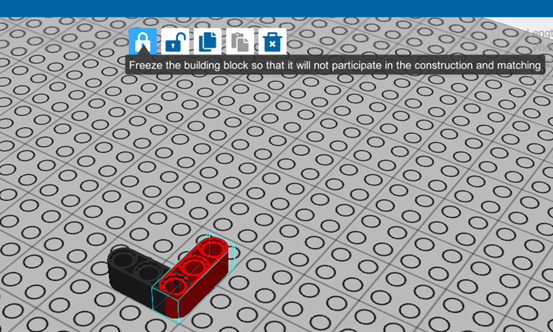
\includegraphics[scale = 0.90]{Imagenes/bloques_constr.png}
    \caption{Bloques en construcción}{Fuente: Propia}
\end{figure}

Lo que significa que se pueden congelar piezas para un mejor control a la hora de construir.
También ofrece un manual para el uso de mouse y teclado

\begin{figure}[H]
    \centering
    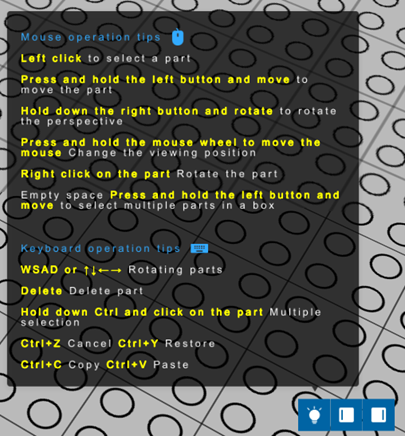
\includegraphics[scale = 0.90]{Imagenes/instruccionesRaton.png}
    \caption{Instrucciones para el uso del ratón en esta interfaz.}{Fuente: Propia}
\end{figure}

Construcción y diseño de espacios para simulación

\begin{figure}[H]
    \centering
    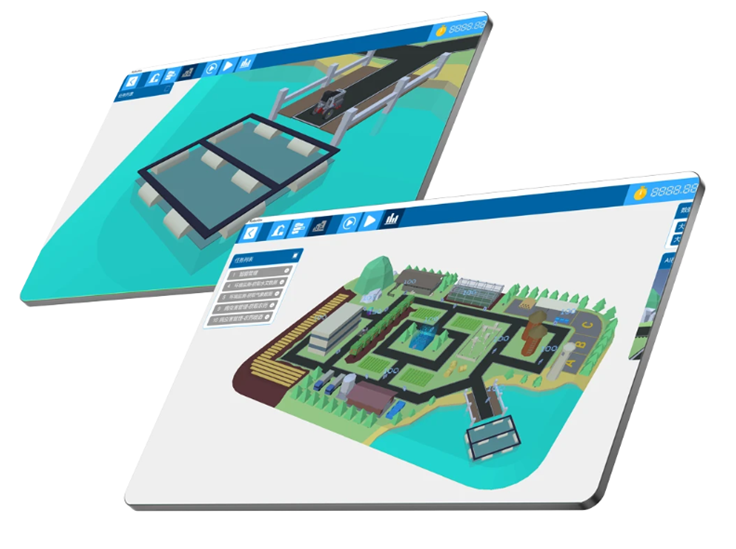
\includegraphics[scale = 0.65]{Imagenes/diseno_entorno.png}
    \caption{Interfaz de Diseño de entorno.}{Fuente: Propia}
\end{figure}

\begin{figure}[H]
    \centering
    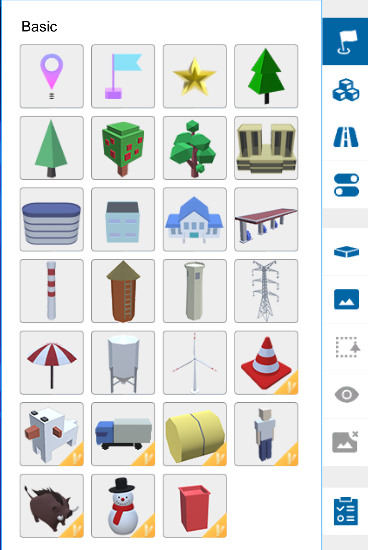
\includegraphics[scale = 0.75]{Imagenes/materiales.png}
    \caption{Materiales para diseño}{Fuente: Propia}
\end{figure}

\begin{figure}[H]
    \centering
    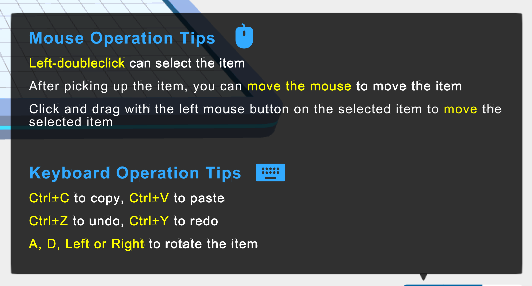
\includegraphics[scale = 0.90]{Imagenes/intr_Raton.png}
    \caption{Guía del uso del ratón}{Fuente: Propia}
\end{figure}

Simulación virtual

\begin{figure}[H]
    \centering
    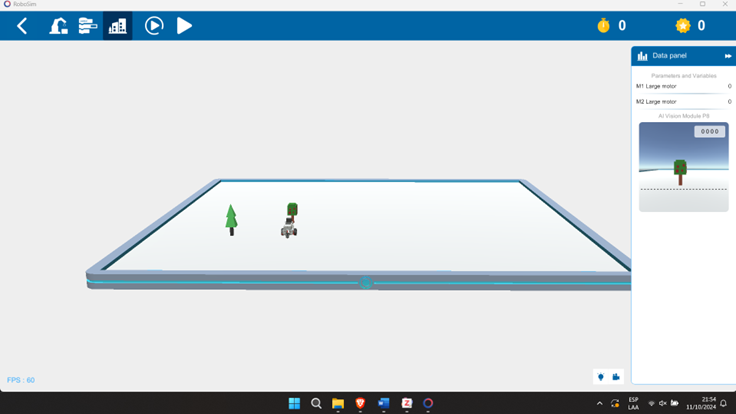
\includegraphics[scale = 0.90]{Imagenes/simulacion_virtual.png}
    \caption{Entorno de simulación virtual}{Fuente: Propia}
\end{figure}

\begin{figure}[H]
    \centering
    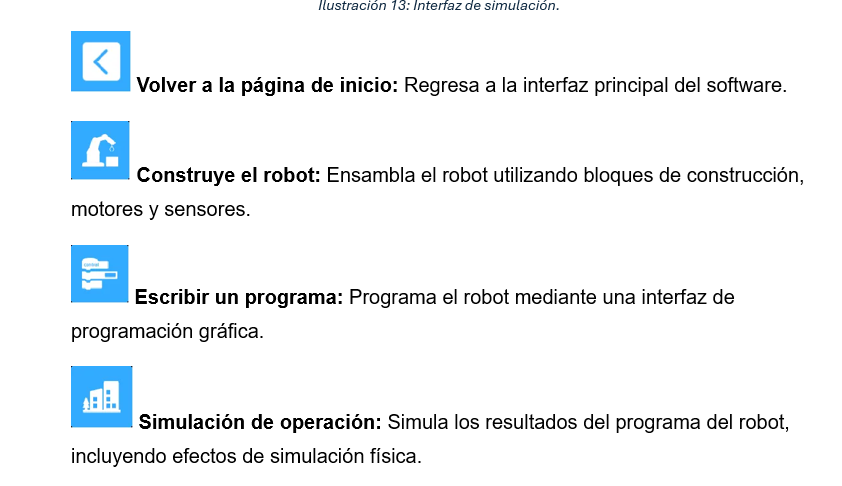
\includegraphics[scale = 0.90]{Imagenes/descripcipn_botones.png}
    \caption{Descripción de botones}{Fuente: Propia}
\end{figure}

Programación

\begin{figure}[H]
    \centering
    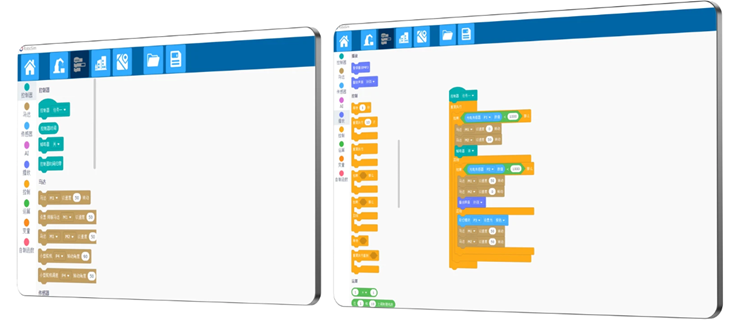
\includegraphics[scale = 0.90]{Imagenes/interfaz_prog.png}
    \caption{Interfaz de programación}{Fuente: Propia}
\end{figure}

\textbf{Tipo de columna:} Divide diferentes módulos de programación en 10 categorías.

\textbf{Módulo de programación:} El módulo de programación correspondiente que controla el robot para ejecutar diferentes instrucciones.

\textbf{Área de programación:} En esta área los módulos de programación se pueden unir para generar un programa de robot.

\textbf{Área de código:} Muestra el código de Python/C++ del programa del robot.

\begin{figure}[H]
    \centering
    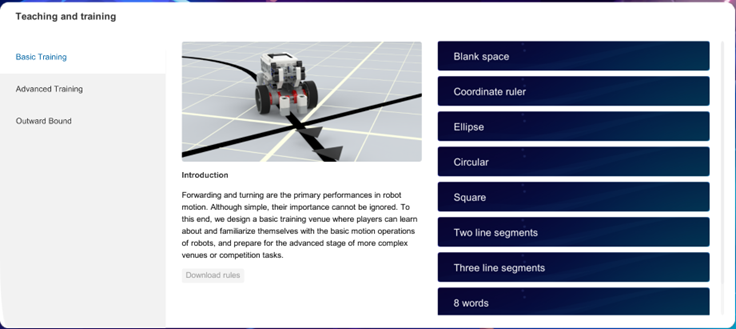
\includegraphics[scale = 0.90]{Imagenes/areas_training.png}
    \caption{Interfaz de entrenamiento}{Fuente: Propia}
\end{figure}

\begin{figure}[H]
    \centering
    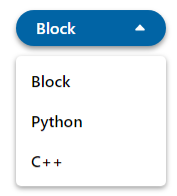
\includegraphics[scale = 0.90]{Imagenes/op_program.png}
    \caption{Tipos de programación y lenguajes}{Fuente: Propia}
\end{figure}

\textbf{Cursos}

\begin{itemize}
    \item \textbf{Curso básico:} Este curso está dirigido principalmente a estudiantes de primaria y secundaria que están expuestos a software de simulación virtual por primera vez. Los estudiantes pueden aprender el proceso de diseño, construcción y programación de robots para simulación en un mundo virtual, y gradualmente adquirir conocimientos sobre operaciones básicas, principios y aplicaciones de sensores, movimiento de robots, estructuras y algoritmos de programación, etc.
    
    \item \textbf{Curso Avanzado:} Dirigido a estudiantes que hayan completado el curso básico. A través de investigaciones entretenidas y proyectos temáticos, los estudiantes no solo consolidarán y reforzarán lo aprendido en la etapa básica, sino que también adquirirán conocimientos multidisciplinarios como movimiento físico, aplicaciones avanzadas de sensores, algoritmos complejos de programación y reconocimiento visual mediante inteligencia artificial.
     
    \item \textbf{Curso de Competencia:} Este curso está diseñado para que los participantes comprendan el proceso de competencias virtuales en línea, los requisitos de reglas, precauciones y claves para completar cada tarea en el recinto temático. Los estudiantes aprenderán habilidades de diseño y programación de robots para competencias basadas en escenarios y conocerán los métodos comunes de depuración y simulación utilizados en la competencia \cite{robosim}.
\end{itemize}

\begin{figure}[H]
    \centering
    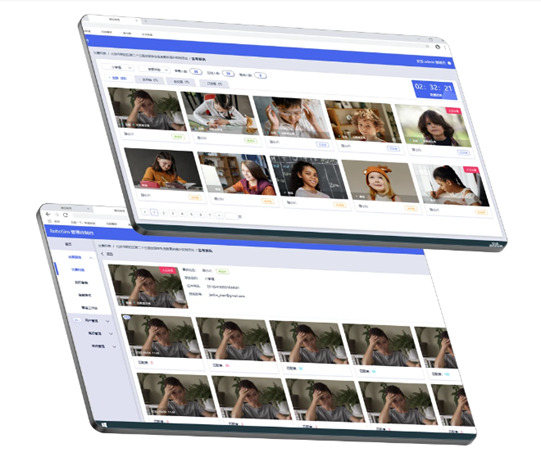
\includegraphics[scale = 0.90]{Imagenes/cursoseduc.png}
    \caption{Cursos educativos disponibles}{Fuente: Propia}
\end{figure}

\textbf{Competencia Online:} Esta plataforma ofrece competición profesional y servicios personalizados.

\begin{figure}[H]
    \centering
    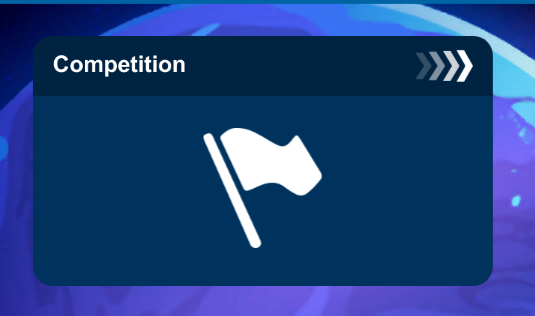
\includegraphics[scale = 0.90]{Imagenes/competir.png}
    \caption{Opción de competición}{Fuente: Propia}
\end{figure}

\begin{figure}[H]
    \centering
    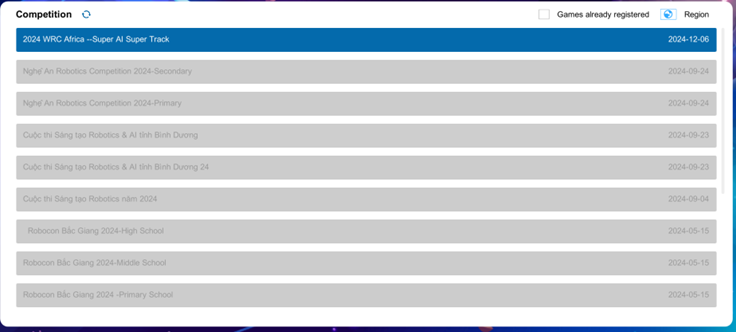
\includegraphics[scale = 0.90]{Imagenes/areas_comp.png}
    \caption{Áreas de competición}{Fuente: Propia}
\end{figure}

\subsection{Ventajas y Desventajas}
\textbf{Las ventajas:}

\begin{itemize}
    \item \textbf{Entorno Seguro de Aprendizaje:} Los usuarios pueden aprender, construir y programar robots en un entorno simulado sin riesgo de dañar equipos o de poner en peligro la seguridad de los estudiantes.
    
    \item \textbf{Variedad de Herramientas Educativas:} Ofrece funcionalidades como la construcción de robots, simulación de competencias, y diseño de entornos de práctica, adaptados a diferentes niveles de habilidad y objetivos de aprendizaje.
    
    \item \textbf{Flexibilidad en el Entrenamiento:} Los usuarios pueden personalizar los entornos de simulación y adaptar sus entrenamientos a diferentes temas o tipos de competencia, lo cual es ideal para quienes desean un aprendizaje autodirigido o enfocado en competencias específicas.
\end{itemize}

\textbf{Desventajas:}

\begin{itemize}
    \item \textbf{Curva de Aprendizaje para Funcionalidades Avanzadas:} Aunque es fácil para principiantes, algunas características avanzadas pueden requerir un tiempo de adaptación, lo cual puede ser un desafío para quienes no tienen conocimientos previos en robótica.
    
    \item \textbf{Dependencia de Recursos Computacionales:} La simulación de efectos físicos y gráficos puede requerir una computadora con buenos recursos (procesador y tarjeta gráfica), lo cual puede limitar el acceso en entornos con computadoras de bajo rendimiento.
    
    \item \textbf{Necesidad de pagar planes:} Esto se presenta como desventaja ya que para hacer uso de algunos recursos de construcción, es necesario pagar algunos de los planes, también el acceso a clases.
\end{itemize}


\subsection{Aplicación}
\textbf{Educación:} Es utilizado en instituciones educativas, como escuelas y universidades, para enseñar robótica, programación y fundamentos de ingeniería. RoboSim permite a los estudiantes experimentar con robots virtuales, desarrollar habilidades prácticas sin necesidad de equipos físicos y comprender conceptos de programación de manera visual e interactiva.

\textbf{Entrenamiento en Competencias de Robótica:} RoboSim es una herramienta ideal para entrenarse en competencias de robótica. Permite a los usuarios participar en desafíos de programación y diseño de robots en línea, preparándolos para competiciones reales sin requerir hardware costoso.

\textbf{Centros de Investigación y Desarrollo:} Aunque RoboSim está orientado a la educación, también puede utilizarse en laboratorios o centros de investigación para prototipado rápido. Los investigadores pueden probar algoritmos de control y modelos de simulación en un entorno virtual antes de aplicarlos a robots físicos.

\textbf{Industria y Capacitación Técnica:} Empresas que implementan robótica en sus operaciones pueden usar RoboSim para capacitar a sus empleados. Esto resulta útil para comprender el funcionamiento y programación de robots industriales en un entorno seguro, permitiendo aprender y resolver problemas de programación y diseño sin riesgos.

\textbf{Desarrollo Personal y Aficionados:} RoboSim también es accesible para aficionados y personas que desean aprender robótica de manera autodidacta. Ofrece un entorno controlado y de bajo costo para experimentar, aprender y desarrollar habilidades en programación de robots.


\subsection{Costos}
Personalización de múltiples versiones, múltiples funciones avanzadas, actualización de la experiencia de servicio
Proporcione servicios profesionales de personalización de múltiples versiones, y la versión de experiencia personal se puede convertir y actualizar a la versión profesional.
También hay una versión de campus, que se puede personalizar de inmediato según las necesidades de la escala regional/escolar.

\begin{figure}[H]
    \centering
    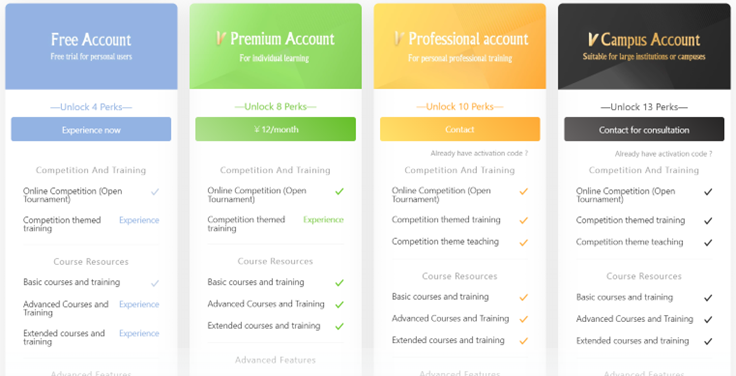
\includegraphics[scale = 0.50]{Imagenes/planes.png}
    \caption{Planes disponibles de Robosim}{Fuente: Propia}
\end{figure}

\newpage
\subsection{Comparación de RoboSim y RoboDK}
\input{comparación_de_robosim_y_robodk.tex}

\chapter{Conclusiones}
Este parcial investigativo y de demostración utilizando RoboSim ha mostrado cómo la simulación se ha convertido en una herramienta clave para el diseño y prueba de sistemas robóticos. Gracias a su capacidad para emular robots sin necesidad de hardware físico, RoboSim permite experimentar con nuevos diseños y algoritmos de forma rápida y segura, reduciendo riesgos y costos asociados a las pruebas físicas. Esto resulta especialmente útil en el desarrollo de robots autónomos, donde las pruebas limitadas al hardware pueden restringir las posibilidades de validación.

Si hablamos a nivel educativo, roboSim ofrece una alternativa efectiva para enseñar robótica y programación, integrando simulaciones que permiten a los estudiantes aprender de manera práctica.
\chapter{Consideraciones Finales}
Considero que este parcial fue interesante porque se explora la herramienta RoboSim como una de tantas para la simulación
de robotica especialmente para un entorno competitivo y educativo. Ver la demostración de mis compañeros y ver las diferencias
entre nuestro software elegido y el de ellos, brinda un enfoque diversificado para simulaciones donde se requiera acciones específicas.

\addcontentsline{toc}{chapter}{Bibliografía}
\begin{thebibliography}{99}
    \bibitem{gucwa cheng}
    \textit{K. J. Gucwa y H. H. Cheng, «RoboSim: A simulated environment for programming modular robots», en 2014 IEEE/ASME 10th International Conference on Mechatronic and Embedded Systems and Applications (MESA), sep. 2014, pp. 1-7. doi: 10.1109/MESA.2014.6935604.}

    \bibitem{zmrobo}
    \textit{«ZMROBO | Education Robot | JoinMax Digital». Accedido: 1 de noviembre de 2024. [En línea].}
    \url{https://www.stemtown.com/about/companyintroduction}

    \bibitem{robosim}
    \textit{«RoboSim». Accedido: 1 de noviembre de 2024. [En línea].}
    \url{https://robosim.stemtown.com/product}

    \bibitem{gucwa2}
    \textit{K. J. Gucwa y H. H. Cheng, «Making Robot Challenges with Virtual Robots», en Proceedings of the 2017 ACM SIGCSE Technical Symposium on Computer Science Education, Seattle Washington USA: ACM, mar. 2017, pp. 273-277. doi: 10.1145/3017680.3017700.}

    \bibitem{zmrobo2}
    \textit{ZMROBO, 1.1.About RoboSim, (14 de noviembre de 2022). Accedido: 1 de noviembre de 2024. [En línea Video]}
    \url{https://www.youtube.com/watch?v=vKZkxZrzepA}

    \bibitem{chino}
    \textit{"Descargar y registrar Yuque" Accedido: 14 de noviembre de 2024. [En línea].}
    \url{https://www.yuque.com/zmrobo/robosim/chn9di}

    \bibitem{simulador}
    \textit{«Simulador para robots industriales y programación fuera línea - RoboDK». Accedido: 14 de noviembre de 2024.}
    \url{https://robodk.com/es/}
\end{thebibliography}
\end{document}
